%%%%%%%%%%%%%%%%%%%%%%%%%%%%%%%%%%%%%%%%%
% University/School Laboratory Report
% LaTeX Template
% Version 3.0 (4/2/13)
%
% This template has been downloaded from:
% http://www.LaTeXTemplates.com
%
% Original author:
% Linux and Unix Users Group at Virginia Tech Wiki 
% (https://vtluug.org/wiki/Example_LaTeX_chem_lab_report)
%
% License:
% CC BY-NC-SA 3.0 (http://creativecommons.org/licenses/by-nc-sa/3.0/)
%
%%%%%%%%%%%%%%%%%%%%%%%%%%%%%%%%%%%%%%%%%

%----------------------------------------------------------------------------------------
%	PACKAGES AND DOCUMENT CONFIGURATIONS
%----------------------------------------------------------------------------------------

\documentclass{article}

\usepackage[version=3]{mhchem} % Package for chemical equation typesetting
\usepackage{siunitx} % Provides the \SI{}{} command for typesetting SI units

\usepackage[top=1in, bottom=1in, right=1in, left=1in]{geometry}

%Add code formating
\usepackage{listings}
\lstset{tabsize=2}

\usepackage{hyperref}

\usepackage{amssymb}

\usepackage{enumerate}

\usepackage{multicol} % Multi-column support

%Add extra support for image placement
\usepackage{float}

\usepackage{mcode}

\usepackage{graphicx} % Required for the inclusion of images

\setlength\parindent{0pt} % Removes all indentation from paragraphs

\renewcommand{\labelenumi}{\alph{enumi}.} % Make numbering in the enumerate environment by letter rather than number (e.g. section 6)

%\usepackage{times} % Uncomment to use the Times New Roman font

% Setup how hyperlinks look
\usepackage{xcolor}
\hypersetup{
	colorlinks,
	linkcolor={red!50!black},
	citecolor={blue!50!black},
	urlcolor={blue!80!black},
}

%----------------------------------------------------------------------------------------
%	DOCUMENT INFORMATION
%----------------------------------------------------------------------------------------

\title{Qt Widget Quick Start} % Title

\author{Blake \textsc{Vermeer}} % Author name

\date{\today} % Date for the report

\begin{document}

\maketitle % Insert the title, author and date

\begin{center}
\begin{tabular}{l r}
Date Performed: & April 3, 2017 \\ % Date the experiment was performed
Company: & Keysight Technologies % Company
\end{tabular}
\end{center}

% If you wish to include an abstract, uncomment the lines below
% \begin{abstract}
% Abstract text
% \end{abstract}

%----------------------------------------------------------------------------------------
%	OVERVIEW
%----------------------------------------------------------------------------------------
\section{Overview}

In this tutorial you will learn how to create a basic Qt Widget application from scratch and deploy it to the Keysight Hacking Platform development kit.



%----------------------------------------------------------------------------------------
%	Create a new Qt Widget Application Project
%----------------------------------------------------------------------------------------
\section{Creating a New Qt Widgets Project}

	\begin{enumerate}[1.)]
		\item First we will use Qt Creator's new project wizard to create a new Qt Widgets project template. First open Qt Creator and then go to \textbf{File $\rightarrow$ New File or Project...}
		
		\item The new project wizard dialog box will pull up. Make sure the \textbf{Generic Linux Device Templates} option is selected in the drop-down menu in the upper right. Select \textbf{Applications} from the left hand menu under projects and then select the \textbf{Qt Widgets Application} project template and then click the \textbf{Choose...} button.
		
			\begin{figure}[H]
				\centering
				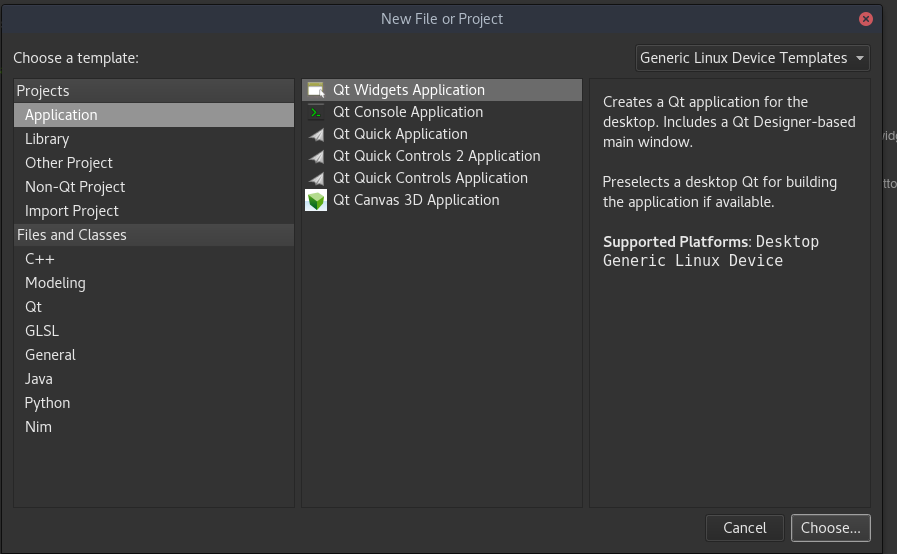
\includegraphics[width=0.85\textwidth]{pics/Choose_Project_Type.png}
				\caption{New Project Wizard Dialog Box}
				\label{Choose_Project_Type}
			\end{figure}
		
		\item In the next dialog box choose a name for the project and where to save it and then click the \textbf{Next} button.
		
			\begin{figure}[H]
				\centering
				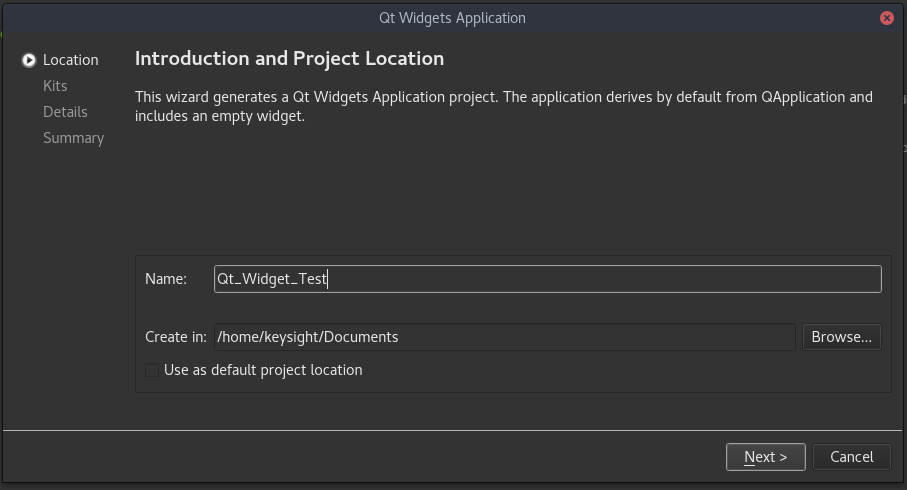
\includegraphics[width=0.85\textwidth]{pics/Name_Project.png}
				\caption{Name the Project}
				\label{Name_Project}
			\end{figure}
		
		\item In the next dialog box make sure that only the \textbf{RPi} box is selected since we are not trying to build a desktop application and then click the \textbf{Next} button.
		
			\begin{figure}[H]
				\centering
				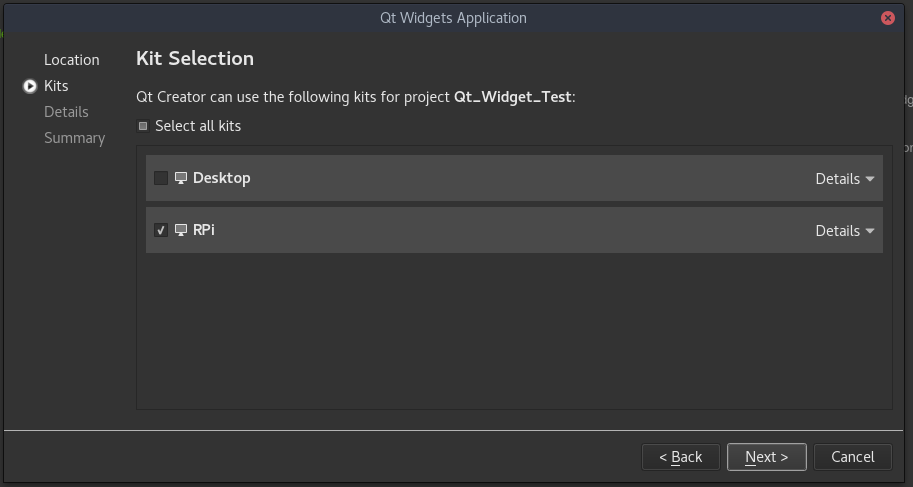
\includegraphics[width=0.85\textwidth]{pics/Kit_Selection.png}
				\caption{Kit Selection}
				\label{Kit_Selection}
			\end{figure}	
		
		\item In the \textbf{Class Information} dialog box leave everything at their default values and click the \textbf{Next} button.
		
			\begin{figure}[H]
				\centering
				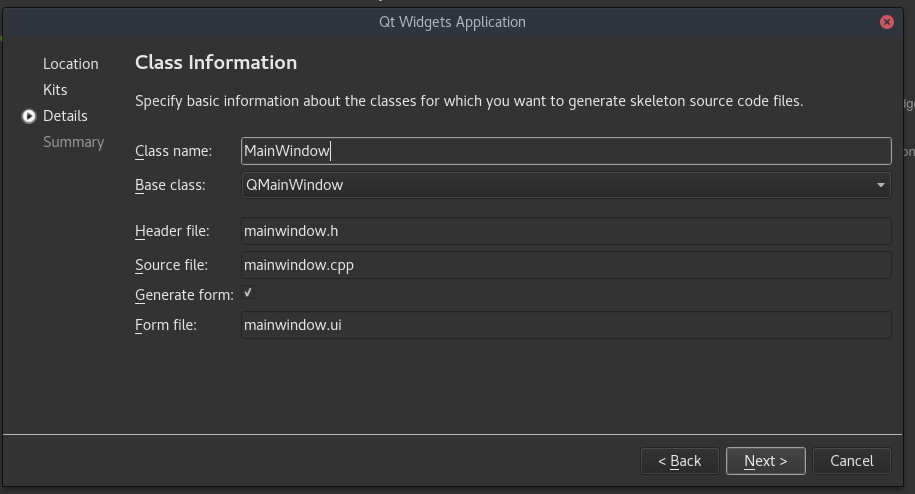
\includegraphics[width=0.85\textwidth]{pics/Class_Info.png}
				\caption{Class Information}
				\label{Class_Info}
			\end{figure}		
		
		\item In the \textbf{Project Management} dialog box leave everything alone and click the \textbf{Finish} button.
		
			\begin{figure}[H]
				\centering
				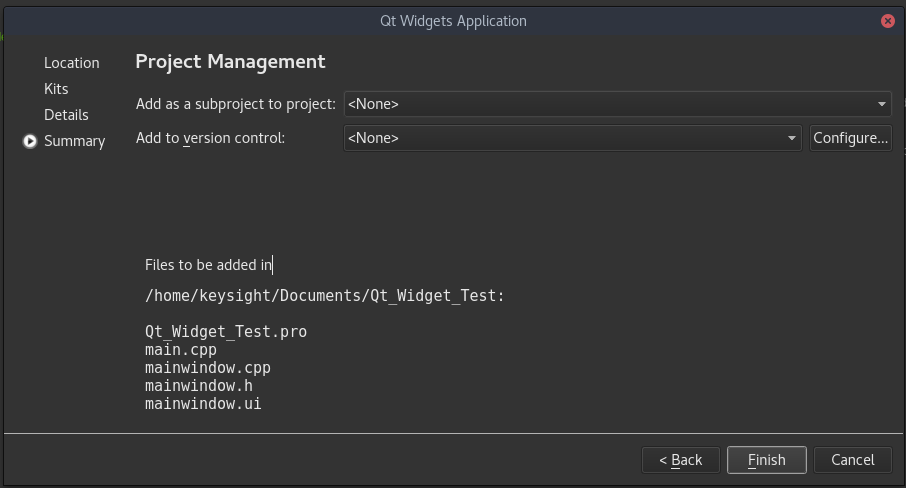
\includegraphics[width=0.85\textwidth]{pics/Project_Management.png}
				\caption{Project Management}
				\label{Project_Management}
			\end{figure}		
		
	\end{enumerate}


%----------------------------------------------------------------------------------------
%	Qt Widgets Project Overview
%----------------------------------------------------------------------------------------
\section{Qt Widgets Project Overview}

The Qt Widgets project wizard creates several different files. This section gives a brief overview of the files created and their purpose.


	\begin{figure}[H]
		\centering
		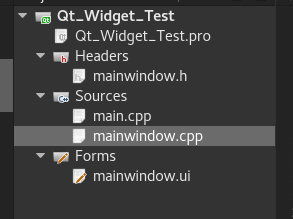
\includegraphics[width=0.25\textwidth]{pics/Project_Files.png}
		\caption{Project Files Created for a Project Name "Qt\_Widget\_Test"}
		\label{Project_Files}
	\end{figure}


Here is a brief overview of the files created for a project called Qt\_Widget\_Test and their purpose:

\begin{itemize}
	\item \textbf{Qt\_Widget\_Test.pro} - The main project file. The project file defines the source files used by the project, the name of the application, where to deploy the application on the target device, and various other settings.
	
	\item \textbf{mainwindow.h} - A header file for the \textit{mainwindow} class. 
	
	\item \textbf{main.cpp} - The main source file for the application. It creates a \textit{QApplication} object need for Qt Widget programs and then creates a \textit{mainwindow} object and displays it.
	
	\item \textbf{mainwindow.cpp} - The source file for the \textit{mainwindow} class. This class inherits from \textit{Q\_OBJECT} and defines the actions done by the various \textit{mainwindow} GUI events.
	
	\item \textbf{mainwindow.ui} - The UI for for the \textit{mainwindow} widget. This file defines the GUI layout for the application.
\end{itemize}


%----------------------------------------------------------------------------------------
%	Preparing the Project File
%----------------------------------------------------------------------------------------
\section{Preparing the Project File}

The default created project file is almost fully complete. The only thing that needs to be added is a target path definition that will tell Qt Creator where to install the application on the target device when deploying it. It is important that the user account you are using on the target device has write access to the target path. Add the three lines as shown in Figure \ref{Target_Path}.

	\begin{figure}[H]
		\centering
		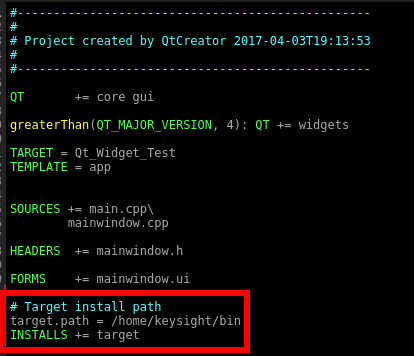
\includegraphics[width=0.5\textwidth]{pics/Add_Target.png}
		\caption{Define the target install path}
		\label{Target_Path}
	\end{figure}


%----------------------------------------------------------------------------------------
%	Creating the GUI
%----------------------------------------------------------------------------------------
\section{Creating the GUI}

This section will explain how to make a basic GUI. Double-click the \textit{mainwindow.ui} file. It will automatically open in the design view.

	\begin{figure}[H]
		\centering
		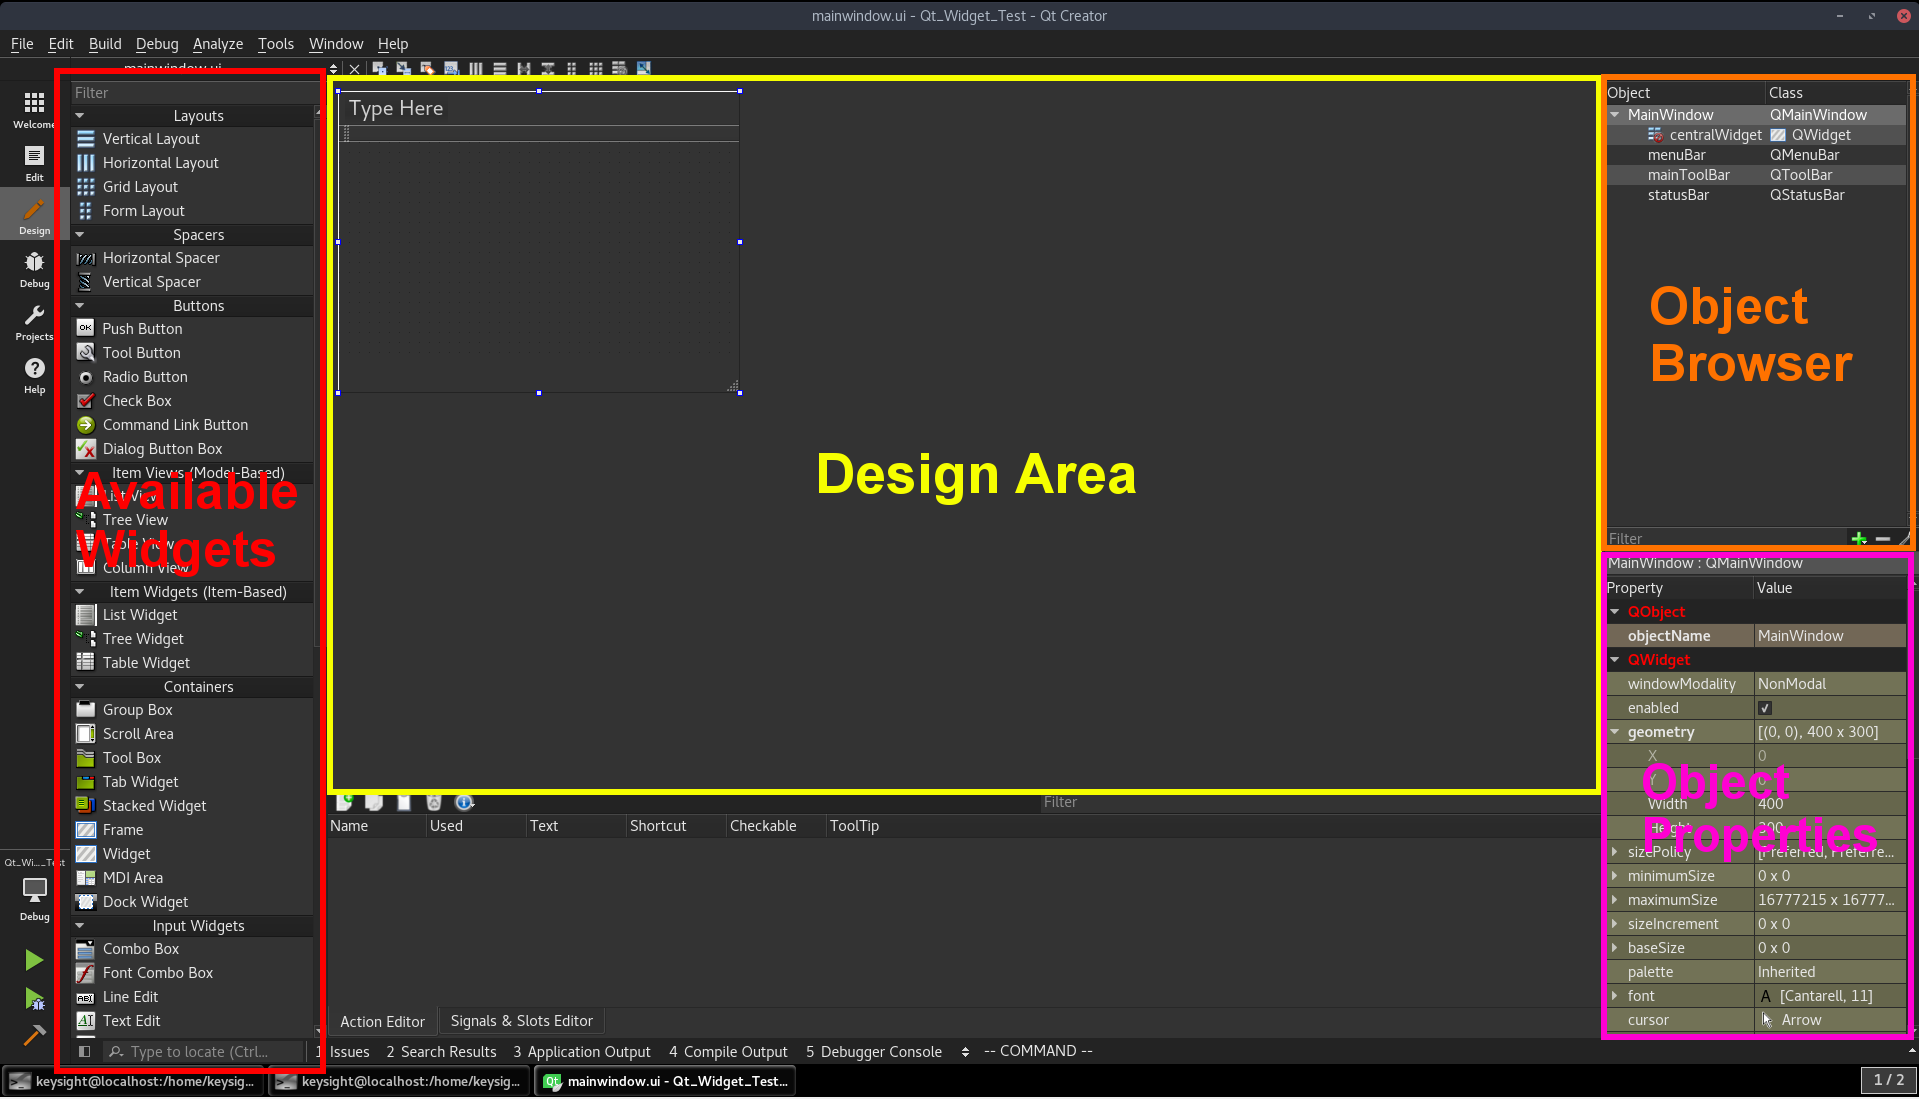
\includegraphics[width=0.85\textwidth]{pics/Qt_Designer.png}
		\caption{Qt Designer Overview}
		\label{Qt_Designer}
	\end{figure}

After opening up the design view the first thing to do is to delete the design objects that are not needed in our UI design. In the \textbf{Object Browser} right-click on the \textbf{statusBar}, \textbf{mainToolBar}, and \textbf{menuBar} object and click remove for each of these. Since we are designing an app which will only run on a device fullscreen with no window manager, we don't need these elements. 

	\begin{figure}[H]
		\centering
		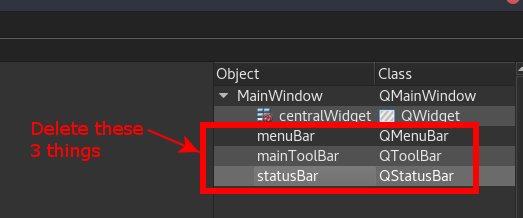
\includegraphics[width=0.5\textwidth]{pics/Delete_Window_Dressings.png}
		\caption{Delete unneeded GUI elements}
		\label{Delete_Window_Dressings}
	\end{figure}

Next we need to change the main window dimensions the the dimensions of our screen. Select the \textbf{MainWindow} from the object browser and then in the object properties dialog box expand the \textbf{geometry} section and change the \textbf{Width to 320} and the \textbf{Height to 240}.

	\begin{figure}[H]
		\centering
		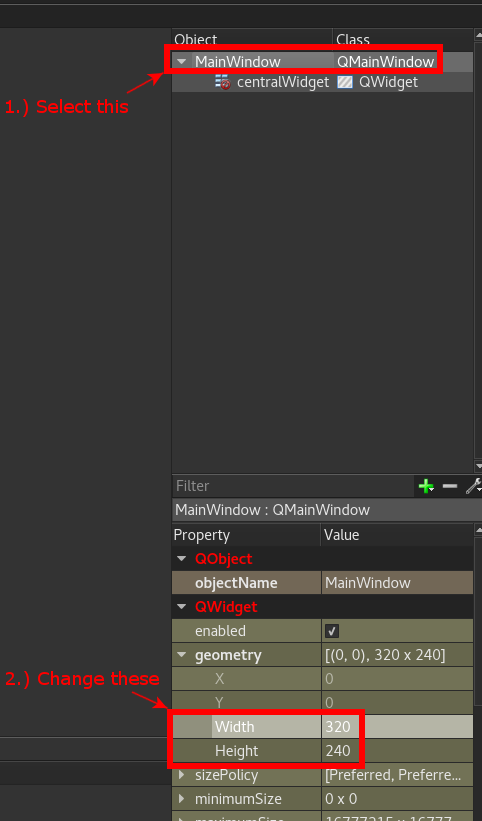
\includegraphics[width=0.35\textwidth]{pics/Set_Geometry.png}
		\caption{Change the main window dimensions to match the screen}
		\label{Set_Geometry}
	\end{figure}

At this point we can choose the color theme for our application. Select the \textbf{MainWindow} from the object browser and then go select \textbf{palette} from the object properties box and then press the \textbf{Change Palette} button next to it.

	\begin{figure}[H]
		\centering
		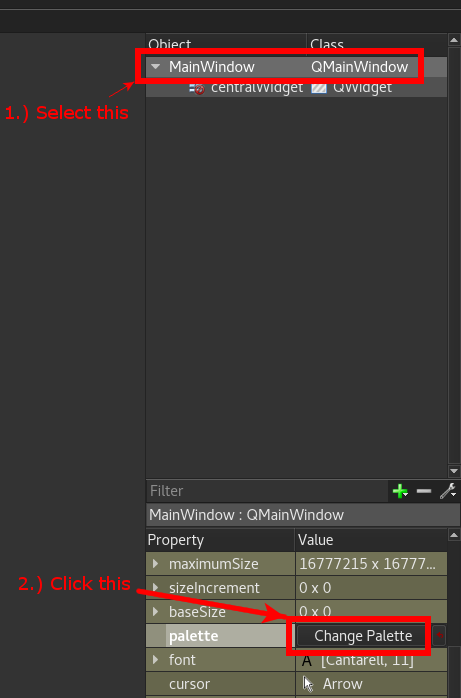
\includegraphics[width=0.35\textwidth]{pics/Change_Palette.png}
		\caption{Change the color scheme for the app}
		\label{Change_Palette}
	\end{figure}

This will pull up the \textbf{Edit Palette} dialog box. From this window you change choose the colors of each individual window element or you can just click on the box to the right of the \textbf{Quick} label and have a color theme automatically generated based on the chosen color. Set up your color scheme and then press OK.

	\begin{figure}[H]
		\centering
		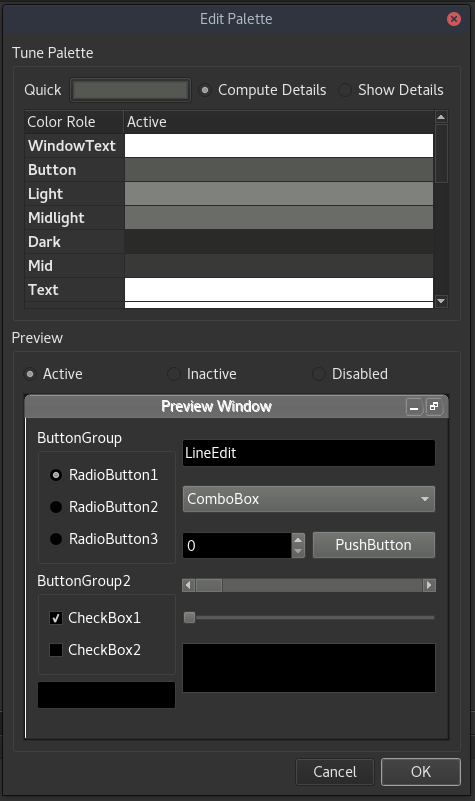
\includegraphics[width=0.35\textwidth]{pics/Edit_Palette.png}
		\caption{Edit the application color scheme}
		\label{Edit_Palette}
	\end{figure}

Now we are going to add three buttons to the UI. Find the \textbf{Push Button} widget in the widget browser and drag three of them to the UI design view. Place them as shown in Figure \ref{Place_Buttons}.

	\begin{figure}[H]
		\centering
		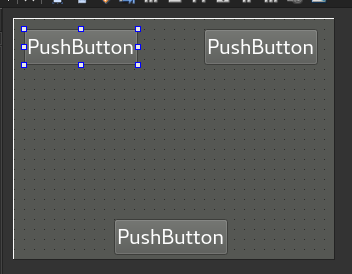
\includegraphics[width=0.35\textwidth]{pics/Place_Push_Buttons.png}
		\caption{Place the push buttons}
		\label{Place_Buttons}
	\end{figure}

Now right-click on the upper left button and choose the \textbf{Change objectName...} option. Rename the upper left button to \textbf{plus\_Button}. Now right-click on the upper left button again and this time choose \textbf{Change text...}. The text on the upper left button to \textbf{+}. Rename and change the text on the other two buttons as shown in Figure \ref{Button_Properties}.

	\begin{figure}[H]
		\centering
		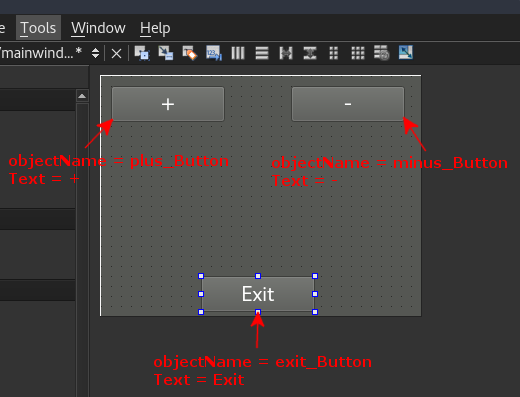
\includegraphics[width=0.5\textwidth]{pics/Button_Properties.png}
		\caption{Set the objectNames and text for the buttons}
		\label{Button_Properties}
	\end{figure}

Now find the \textbf{LCD Number} widget from the widget browser and drag it to the middle of the UI as shown in Figure \ref{Add_LCD}. Resize the LCD display as you see fit. 

	\begin{figure}[H]
		\centering
		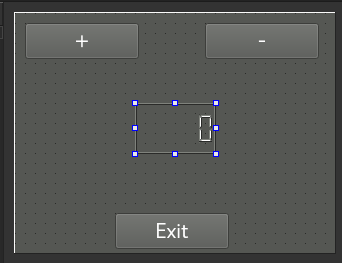
\includegraphics[width=0.5\textwidth]{pics/Add_LCD.png}
		\caption{Add a LCD widget to the UI}
		\label{Add_LCD}
	\end{figure}


%----------------------------------------------------------------------------------------
%	Create Button Signals
%----------------------------------------------------------------------------------------
\section{Create Button Signals}

Now we are going to change the design view to the \textbf{Edit Signals/Slots} view to edit the events that are called when the buttons are pressed. In the bar directly above the design area click the \textbf{Edit Signals/Slots} button as shown in Figure \ref{Signals_Button}. 

	\begin{figure}[H]
		\centering
		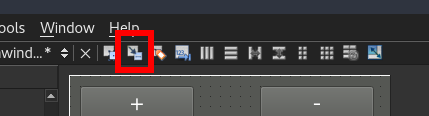
\includegraphics[width=0.5\textwidth]{pics/Signals_Button.png}
		\caption{Edit Signals/Slot Button}
		\label{Signals_Button}
	\end{figure}

Click and drag from the exit button until a red wire with a ground symbol appears and then release your mouse. This will bring up a \textbf{Configure Connection} dialog box for the \textbf{Exit} button.

	\begin{figure}[H]
		\centering
		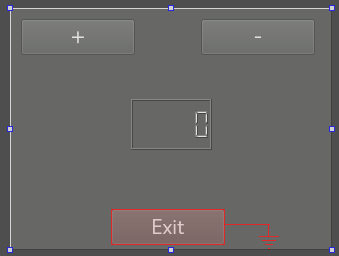
\includegraphics[width=0.5\textwidth]{pics/Exit_Signal.png}
		\caption{Create a new signal for the Exit button}
		\label{Exit_Signal}
	\end{figure}

In the \textbf{Configure Connection} dialog box choose \textbf{clicked()} for the exit\_Button signal, then check the box to 'Show signals and slots inherited from QWidget', and then choose \textbf{close()} for the event. This will cause the application to close when the exit button is pressed.

	\begin{figure}[H]
		\centering
		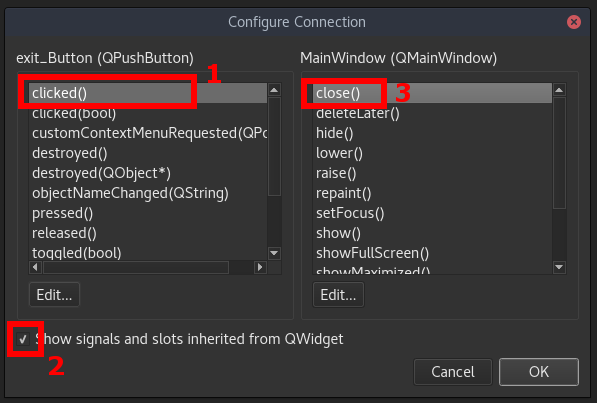
\includegraphics[width=0.5\textwidth]{pics/Configure_Exit.png}
		\caption{Set the Exit button to close the application}
		\label{Configure_Exit}
	\end{figure}

Now we will go back to the \textbf{Edit Widgets} view by clicking the \textbf{Edit Widgets} button in the toolbar above the design area to add signal function stubs for the other two buttons.

	\begin{figure}[H]
		\centering
		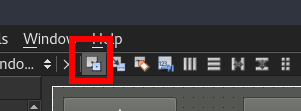
\includegraphics[width=0.5\textwidth]{pics/Edit_Widgets.png}
		\caption{Switch back to Edit Widgets mode}
		\label{Edit_Widgets}
	\end{figure}

Now select the \textbf{Plus Button} and right click it and choose \textbf{Go to slot...}. This will pull up a dialog box and in it select the \textbf{clicked()} signal and then press OK. This will create a function stub for us in the MainWindow class that is called when the plus button is clicked.

	\begin{figure}[H]
		\centering
		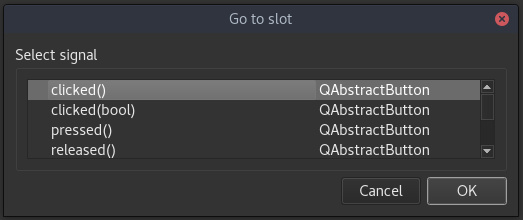
\includegraphics[width=0.5\textwidth]{pics/Go_to_Slot.png}
		\caption{Go to slot dialog}
		\label{Go_to_Slot}
	\end{figure}

	\begin{figure}[H]
		\centering
		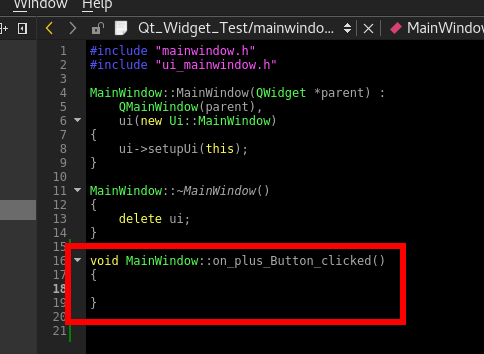
\includegraphics[width=0.5\textwidth]{pics/New_Signal.png}
		\caption{New signal function stub}
		\label{New_Signal}
	\end{figure}

For now leave the function stub alone and double-click on the \textbf{mainwindow.ui} file under Forms to go back to the GUI designer.

	\begin{figure}[H]
		\centering
		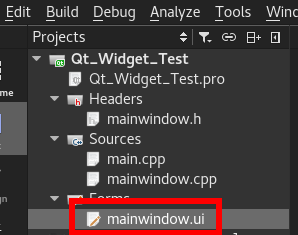
\includegraphics[width=0.5\textwidth]{pics/UI_File.png}
		\caption{Go back to editing the UI file}
		\label{UI_File}
	\end{figure}

Right-click on the \textbf{minus button} and click \textbf{Go to slot...} and chose the clicked option similar to what was done with the plus button. At this point you should be seeing the \textbf{mainwindow.cpp} file and it should look like Figure \ref{Empty_Button_Slots}.

	\begin{figure}[H]
		\centering
		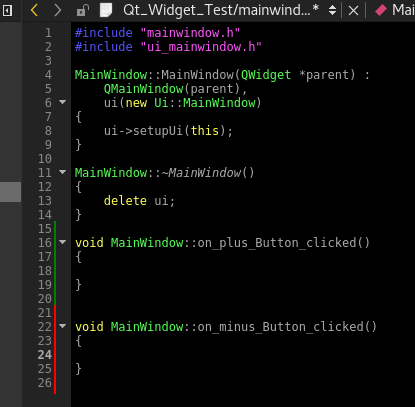
\includegraphics[width=0.5\textwidth]{pics/Empty_Button_Slots.png}
		\caption{mainwindow.cpp with function prototypes for the buttons}
		\label{Empty_Button_Slots}
	\end{figure}

Now double-click the \textbf{mainwindow.h} file to open it. Add a new private variable to keep track of the LCD display number as shown in Figure \ref{lcd_val}.

	\begin{figure}[H]
		\centering
		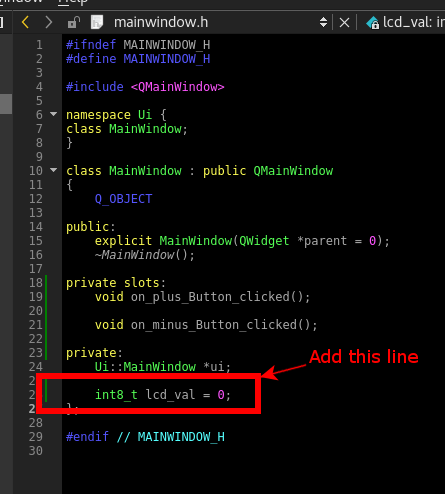
\includegraphics[width=0.5\textwidth]{pics/lcd_val.png}
		\caption{Add a private variable called lcd\_val}
		\label{lcd_val}
	\end{figure}

Now double-click on the \textbf{mainwindow.cpp} file to open in again. Fill out the button function as shown in Figure \ref{Complete_Button_Functions}.

	\begin{figure}[H]
		\centering
		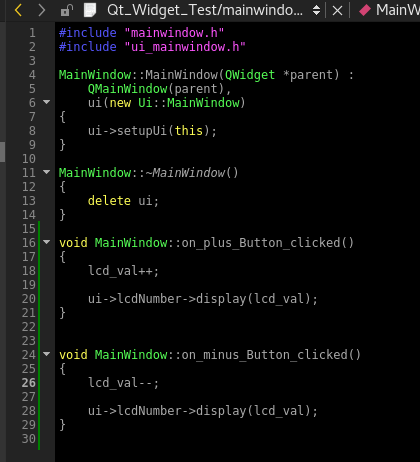
\includegraphics[width=0.5\textwidth]{pics/Complete_Button_Functions.png}
		\caption{Completed button functions}
		\label{Complete_Button_Functions}
	\end{figure}

At this point the program is complete and is ready to be deployed to the Raspberry Pi to be tested. Click the \textbf{Start Debugging} button in the lower left hand side of the screen (or press the F5 key) to deploy the application to the Raspberry Pi and open up a debugging session for the application.

	\begin{figure}[H]
		\centering
		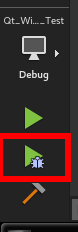
\includegraphics[width=0.1\textwidth]{pics/Start_Debug_Button.png}
		\caption{Start Debugging Button}
		\label{Start_Debug_Button}
	\end{figure}




%----------------------------------------------------------------------------------------
%	APPENDIX
%----------------------------------------------------------------------------------------

%\newpage
%\section{Appendix}

%\begin{enumerate}

	
%	\item[1. a.)] \lstinputlisting{../MATLAB/problem_1a.m}
	

%\end{enumerate}






%----------------------------------------------------------------------------------------


\end{document}